\documentclass{beamer}        
\usetheme[compress]{Berlin}
\usecolortheme{dove}
\usepackage{time}            
\usepackage{graphicx}
\usepackage{graphics}
\usepackage[T1]{fontenc}    
\usepackage{amssymb,amsmath} 
\usepackage{palatino}
\definecolor{links}{HTML}{2A1B81}
\hypersetup{colorlinks,linkcolor=,urlcolor=links}
\DeclareMathOperator*{\E}{\mathbb{E}}
\DeclareMathOperator*{\argmax}{arg\,max}

\title{[POLS 8500] Introduction to Statistical Learning Theory}
\author{Professor Jason Anastasopoulos\\
			\href{ljanastas@uga.edu}{ljanastas@uga.edu}}
\institute{University of Georgia
			}
\date{January 19, 2017}
\setbeamercovered{transparent}

\begin{document}

\begin{frame} % Slide 1
\titlepage
\end{frame}


\section*{Outline}

\begin{frame}{For today...} 
	\begin{itemize}
	 	\item What is statistical learning?
	 	\item Statistics in social science -- causality.
	 	\item Statistics in machine learning -- prediction.
	 	\item	Reducible and irreducible errors.
	 	\item Estimating $f$. 
	 	\item Accuracy v. interpretability.
	 	\item Model accuracy.
	 	\item The bias-variance tradeoff.
	 	\item Classification.
	\end{itemize}
\end{frame}

\section*{Statistical learning}

\begin{frame}{Statistical learning theory} % Slide 2

 \begin{itemize}
 	\item \textit{Input variables} -- $\mathcal{X}$.
 		\begin{itemize}
 			\item AKA features, independent variables, predictors, etc..
 		\end{itemize}
 	\item \textit{Output variables.} -- $\mathcal{Y}$.
 				\begin{itemize}
 			\item AKA dependent variables, outcomes, etc.
 		\end{itemize}
 	\item Eg) Advertising expenditures.
 \end{itemize}
\end{frame}

\begin{frame}{Statistical learning theory} % Slide 2
\begin{align*}
	f: \mathcal{X} &\rightarrow \mathcal{Y} \\
	 \mathcal{X} \in \mathbb{R}^{nxp} & ; \mathcal{Y}  \in \mathbb{R}^{p} \\
\end{align*}

 \begin{itemize}
 	\item Abstractly is find a function $f$ that accurately maps the inputs $\mathcal{X}$ to outputs $\mathcal{Y}$
 	
 \end{itemize}
\end{frame}

\begin{frame}{Statistical learning theory} % Slide 2
\begin{align*}
	 Y = f(X) + \epsilon
\end{align*}

 \begin{itemize}
 	\item More concretely, we are interested in finding a function $f(X)$ which can return values of an output $Y$.
 	\item In introduction to regression courses, this is typically the equation you see.
    \item $f(X)$ is an unknown function of a matrix of predictors $X = (X_{1},\cdots, X_{p})$, an outcome $Y$ and an error term $\epsilon$.
 \end{itemize}
\end{frame}


\section*{Statistics}

\subsection*{Social science -- causality}

\begin{frame}{Approach in social science} % Slide 2
\begin{align*}
	 Y = f(X) + \epsilon
\end{align*}

 \begin{itemize}
 	\item While $X$ and $Y$ are known, $f(\cdot)$ is unknown.
 	\item The goal of statistical learning, then, is to utilize a set of approaches to estimate the ``best'' $f(\cdot)$ for the problem at hand.
 \end{itemize}
\end{frame}

\begin{frame}{Statistical learning theory} % Slide 2
\begin{align*}
	 f(X) = & \sum_{i=1}^{p} \beta_{i} x_{i} \\
	 \epsilon \sim &  N(0, \sigma^{2}) \\ 
	 Y = & \sum_{i=1}^{p} \beta_{i} x_{i} + \epsilon
\end{align*}

 \begin{itemize}
 	\item In social science, we often choose a linear function to estimate $Y$ and assume that the error term is normally distributed with a zero mean.
 	\item Parameters $\beta$ are estimated by minimizing the sum of squared errors which form the normal equations $(\mathbf{X}^{T}\mathbf{X})^{-1} \mathbf{X}^{T} Y$
 \end{itemize}
\end{frame}


\begin{frame}{Approach in social science: causality} % Slide 2
\begin{align*}
	 Y = \beta_{0} + \beta_{1} T + \sum_{i = i}^{p-1} \beta_{i} x_{i} + \epsilon
\end{align*}

 \begin{itemize}
 	\item Often we are interested in the values of one or two parameters and whether they are \textit{causal} or not.
 	\item There are many interpretations of statistical causality (ie Pearl (2009), Rubin (1974)). 
 	\item The general idea is that $\beta_{1}$ measures the extent to which $\Delta X_{t}$ will affect $\Delta Y_{t+1}$.
 \end{itemize}
\end{frame}


\begin{frame}{Approach in social science: causality} % Slide 2
\begin{align*}
	 Y = \beta_{0} + \beta_{1} T + \sum_{i = i}^{p-1} \beta_{i} x_{i} + \epsilon
\end{align*}

 \begin{itemize}
 	\item Causal inference requires that $ T \perp \epsilon$ or $ T| X \perp \epsilon $.
 	\item This often requires \textit{randomization} of $T$ under most circumstances.
 	\item This implies that we are not really all that interested in choosing an optimal $f(\cdot)$.
 \end{itemize}
\end{frame}


\begin{frame}{Approach in social science: causality} % Slide 2
\begin{align*}
\text{Choose design: }& 	\delta \subset \Delta \\
\text{s.t.: } & \exists x_{i} \in \mathbf{X} \\
\text{satisfying: } &  x_{i} \perp \epsilon 
\end{align*}

 \begin{itemize}
 	\item Choose a subset of research designs $\delta$ from all possible designs $\Delta$ so that you have at least one treatment (variable) that is randomized. 
 \end{itemize}
\end{frame}

\subsection*{Machine learning -- prediction}

\begin{frame}{Approach in machine learning: prediction} % 
\begin{align*}
		\hat{Y} = \hat{f(}X)
\end{align*}

 \begin{itemize}
 	\item Machine learning is primarily concerned with prediction.
 	\item We are interested in finding the ``best'' $f(\cdot)$ and the ``best'' set of $X$'s which give the best predictions, $\hat{Y}$.
 	\item We want to find the function that minimize the difference between the \textit{predicted} values and the \textit{observed} values.
 \end{itemize}
\end{frame}

\section*{Error}

\begin{frame}{Reducible and irreducible error} % 
\begin{align*}
		\hat{f}(X) & = \hat{Y} & \text{ estimated function} \\
		 f(X) + \epsilon  & = Y  & \text{ true function} 
\end{align*}

 \begin{itemize}
 		\item Prediction of $Y$ with $\hat{Y}$ can be broken down into two components: reducible and irreducible error.
 		\item \textbf{reducible error} -- $\hat{f}$ is used to estimate $f$ but is not perfect. Improving the accuracy of $\hat{f}$ can be accomplished by adding more \textit{observed} features (variables) to the model.
 		\item \textbf{irreducible error} -- $\epsilon$ represents all other features that can be used predict $f$. These are unobserved and thus are irreducible.
 \end{itemize}
\end{frame}

\begin{frame}{Reducible and irreducible error} % 
\begin{align*}
		\mathbb{E}(Y-\hat{Y})^{2} & = \mathbb{E}[ f(X) + \epsilon - \hat{f}(X)]^{2} \\
			     				 & = \mathbb{E}[(f(X) + \epsilon - \hat{f}(X))(f(X) + \epsilon - \hat{f}(X))] \\
			     				 & = [f(X) - \hat{f}(X)]^{2} + Var(\epsilon)
\end{align*}

\end{frame}


\section*{Estimating $f$}

\begin{frame}{Estimating \textit{f}} % 

\begin{itemize}
	\item \textbf{Training data} -- is required to ``teach'' our machine learning algorithm to predict outcomes. 
	\item \textit{Predicting presidential elections}
		\begin{itemize}
			\item \textbf{outcome/Response}- presidential candidate vote share in each state for the Republican candidate.
			\item \textbf{features} -- state Republican vote share in last election, ?.
		\end{itemize}
\end{itemize}

\end{frame}


\begin{frame}{Estimating \textit{f} -- example 1 -- predicting elections} % 
	\begin{align*}
	\text{Training data: }	\{(x_{1},y_{1}), & (x_{2},y_{2}), \cdots, (x_{n},y_{n}) \} \\ 
		x_{i} = & (x_{i1}, x_{i2}, \cdots, x_{ip})^{T} 
	\end{align*}

\begin{itemize}
	\item $n = 50$ states.
	\item $i = 1,\cdots,n$ observations (states), $j = 1,\cdots,p$ features (state-level variables).
	\item Training data: feature (or feature set) $x_{ip}$ and outcome $y_{i}$ (election results).
\end{itemize}

\end{frame}


\begin{frame}{Estimating \textit{f} -- example 2 --  political sentiment  in Tweets} % 
	\begin{align*}
	\text{Training data: }	\{(x_{1},y_{1}), & (x_{2},y_{2}), \cdots, (x_{n},y_{n}) \} \\ 
		x_{i} = & (x_{i1}, x_{i2}, \cdots, x_{ip})^{T}
	\end{align*}

\begin{itemize}
	\item $n = 1,000$ Tweets.
	\item $i = 1,\cdots,n$ observations (Tweets), $j = 1,\cdots,p$ features (words, tweet length, etc).
	\item Training data: feature (or feature set) $x_{ip}$ and outcome $y_{i}$ (pro/anti Trump).
\end{itemize}

\end{frame}


\begin{frame}{Estimating \textit{f} -- parametric methods} % 
\begin{align*}
	\text{Step 1 -- Functional form: } & f(X) = \beta_{0} + \sum_{i=1}^{p}\beta_{i} x_{i} \\
	\text{Step 2 -- Training: } & Y = \beta_{0} + \sum_{i=1}^{p}\beta_{i} x_{i}
\end{align*}
	\begin{itemize}
		\item \textit{parametric methods} are model-based approaches that involve two steps.
		\item \textbf{step 1} involves choosing a predefined functional form. Linear, quadratic, etc. 
		\item \textbf{step 2} involves \textit{training} or fitting the model using the training data.
	\end{itemize}

\end{frame}


\begin{frame}{Estimating \textit{f} -- parametric methods -- issues} % 
\begin{align*}
Y = \beta_{0} + \sum_{i=1}^{p}\beta_{i} x_{i} + & \sum_{i=1}^{p} +  \\  
 \beta_{i} x_{i}^{2} + & \sum_{i=1}^{p}\beta_{i} x_{i}^{3} + \cdots
\end{align*}
	\begin{itemize}
		\item Rigid models such as a strictly linear model may not fit the data well.
		\item More flexible models require more parameter estimation and may result in \textbf{overfitting} -- a model that is only useful for the training data at hand.
	\end{itemize}

\end{frame}


\begin{frame}{Estimating \textit{f} -- parametric methods -- examples} % 
\centering
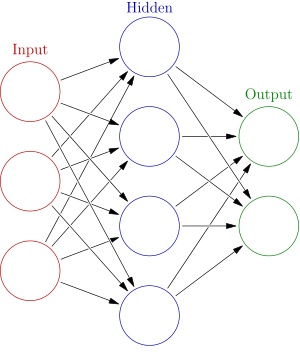
\includegraphics[scale=.35]{neuralnets}
	\begin{itemize}
	\item Linear regression.
	\item Logistic regression.
	\item Naive bayes.
	\item Neural networks.
	\end{itemize}

\end{frame}


\begin{frame}{Estimating \textit{f} -- non-parametric methods} % 
	\begin{itemize}
		\item \textbf{non-parametric} methods do not assume anything about the functional form of \textit{f}. 
		\item Estimates a function only based on the data itself.
	\end{itemize}

\end{frame}


\begin{frame}{Estimating \textit{f} -- non-parametric methods -- examples} % 
\centering
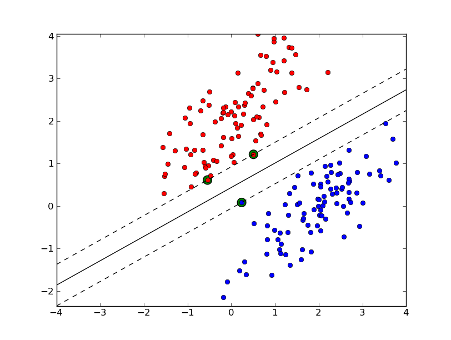
\includegraphics[scale=.45]{svms}
	\begin{itemize}
		\item K-Nearest Neighbors.
		\item Support vector machines.
		\item Decision trees.
	\end{itemize}

\end{frame}

\subsection*{Accuracy v. interpretability}

\begin{frame}{Accuracy and interpretability tradeoffs} % 
\centering
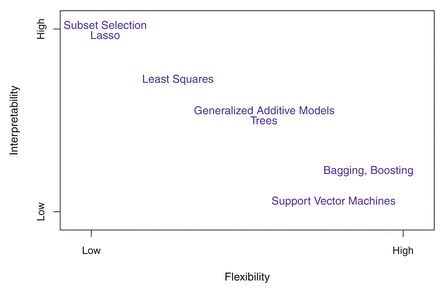
\includegraphics[scale=.45]{flexibility}
	\begin{itemize}
		\item More accurate models often require estimating more parameters and/or having more flexible models.
		\item More models that are better at prediction generally are less interpretable.
	\end{itemize}

\end{frame}



\begin{frame}{Supervised v. unsupervised learning } % 
	\begin{itemize}
		\item \textbf{Supervised learning} involves estimating functions with known observation and outcome data.
		\item \textbf{Unsupervised learning} involves estimating functions without the aid of outcome data. 
	\end{itemize}

\end{frame}


\begin{frame}{Supervised learning -- examples } % 
	\begin{itemize}
		\item Naive bayes.
		\item Support vector machines.
		\item Neural networks.
		\item Linear regression.
	\end{itemize}
\end{frame}

\begin{frame}{Unsupervised learning -- examples } % 
\centering
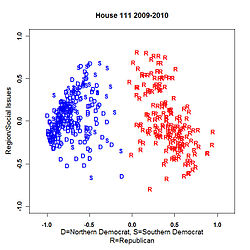
\includegraphics[scale=.5]{nominate}
	\begin{itemize}
		\item Topic models.
		\item K-Means clustering.
		\item Multidimensional scaling.
		\item Pagerank.
	\end{itemize}
\end{frame}

\begin{frame}{Unsupervised learning -- examples } % 
\centering
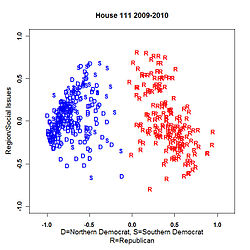
\includegraphics[scale=.5]{nominate}
	\begin{itemize}
		\item Topic models.
		\item K-Means clustering.
		\item Multidimensional scaling.
		\item Pagerank.
	\end{itemize}
\end{frame}

\subsection*{Model accuracy}

\begin{frame}{Assessing model accuracy } % 
	\begin{itemize}
		\item Machine learning is as much an art as it is a science.
		\item There is not best method, only a method that best fits a problem.
	\end{itemize}
\end{frame}

\begin{frame}{Measuring fit } %
\begin{align*}
	MSE = \frac{1}{n} \sum_{i = 1}^{n} (y_{i} - \hat{f} (x_{i}) )^{2}
\end{align*} 
	\begin{itemize}
		\item In the regression setting, the mean squared error is a metric of how well a model fits the data. 
		\item To estimate model fit we need to partition the data:
			\begin{enumerate}
				\item Training set -- data that we will use to fit the model.
				\item Test set -- data that we will use to test the fit of the model.
			\end{enumerate}
	\end{itemize}
\end{frame}


\begin{frame}{Measuring fit } %
\begin{align*}
	MSE = \frac{1}{n} \sum_{i = 1}^{n} (y_{i} - \hat{f} (x_{i}) )^{2}
\end{align*} 
	\begin{itemize}
		\item \textbf{Training MSE} tells us how well our model fits the training data.
		\item \textbf{Test MSE} tells us  how well our  model fits new data.
		\item We are most concerned in minimizing \textit{test MSE}.
	\end{itemize}
\end{frame}

\begin{frame}{How to choose training and test set? } %

	\begin{itemize}
		\item Divide labeled data randomly into two parts: training and test sets.
		\item \textbf{Cross-validation} involves randomly dividing the data into training and test sets several times and assessing the \textit{average} model fit across each test set.
	\end{itemize}
\end{frame}

\begin{frame}{Training MSE, test MSE and model flexibility}
 \centering
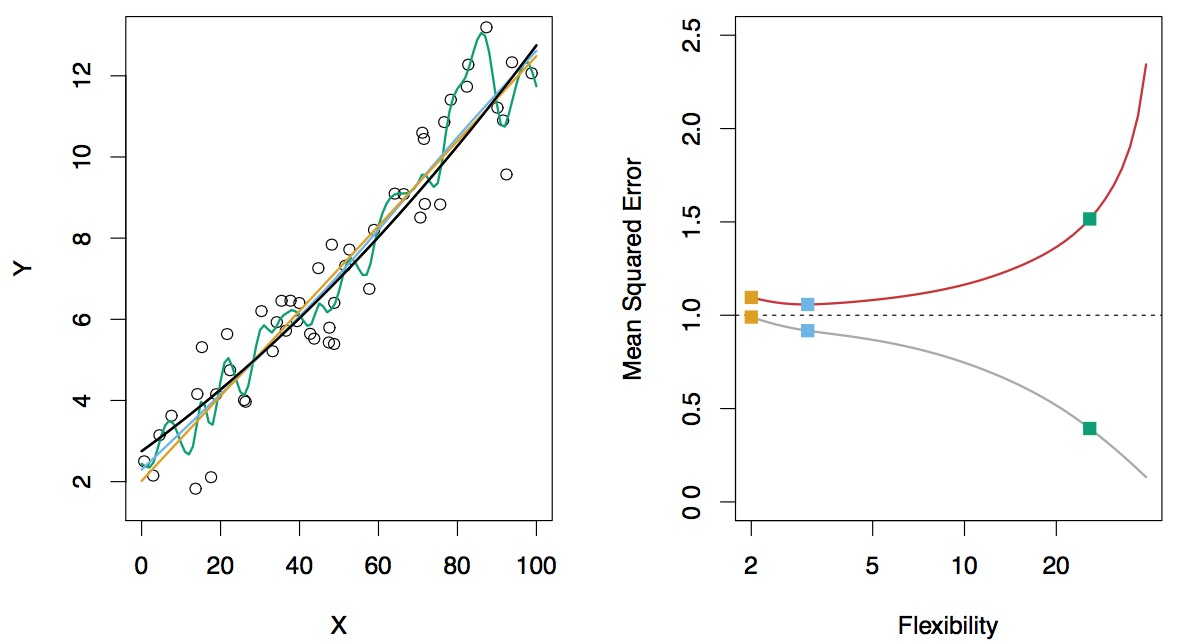
\includegraphics[scale=.2]{trainingtest}

	\begin{itemize}
		\item Increasing model flexibility tends to \textit{decrease} training MSE but will eventually \textit{increase} test MSE.
	\end{itemize}
\end{frame}


\section*{Bias-variance tradeoff}

\begin{frame}{The bias-variance tradeoff}
\begin{align*}
	\mathbb{E} (y_{0} - \hat{f}(x_{0}))^{2} = Var(\hat{f}(x_{0})) + [\text{Bias}(\hat{f}(x_{0})]^{2} + Var(\epsilon)
\end{align*}
	\begin{itemize}
		\item It can be shown that the expected value for the test MSE can be decomposed into 3 components:
			\begin{enumerate}
				\item $Var(\hat{f}(x_{0}))$ -- Variance of the predictions.
				\item $ [\text{Bias}(\hat{f}(x_{0})]^{2}$ -- Bias of the predictions.
				\item $Var(\epsilon)$ -- Variance of the error terms.
			\end{enumerate}
	\end{itemize}
\end{frame}

\begin{frame}{The bias-variance tradeoff}
\begin{align*}
	\mathbb{E} (y_{0} - \hat{f}(x_{0}))^{2} = Var(\hat{f}(x_{0})) + [\text{Bias}(\hat{f}(x_{0})]^{2} + Var(\epsilon)
\end{align*}
	\begin{itemize}
		\item It can be shown that the expected value for the test MSE can be decomposed into 3 components:
			\begin{enumerate}
				\item $Var(\hat{f}(x_{0}))$ -- how much would $\hat{f}$ change if we applied it to a different data set.
				\item $ [\text{Bias}(\hat{f}(x_{0})]^{2}$ -- how well does the model fit the data?
			\end{enumerate}
	\end{itemize}
\end{frame}

\begin{frame}{The bias-variance tradeoff}
\begin{align*}
	\mathbb{E} (y_{0} - \hat{f}(x_{0}))^{2} = Var(\hat{f}(x_{0})) + [\text{Bias}(\hat{f}(x_{0})]^{2} + Var(\epsilon)
\end{align*}
	\begin{itemize}
		\item It can be shown that the expected value for the test MSE can be decomposed into 3 components:
			\begin{enumerate}
				\item $Var(\hat{f}(x_{0}))$ -- how much would $\hat{f}$ change if we applied it to a different data set.
				\item $ [\text{Bias}(\hat{f}(x_{0})]^{2}$ -- how well does the model fit the data?
			\end{enumerate}
	\end{itemize}
\end{frame}


\begin{frame}{The bias-variance tradeoff}
\centering
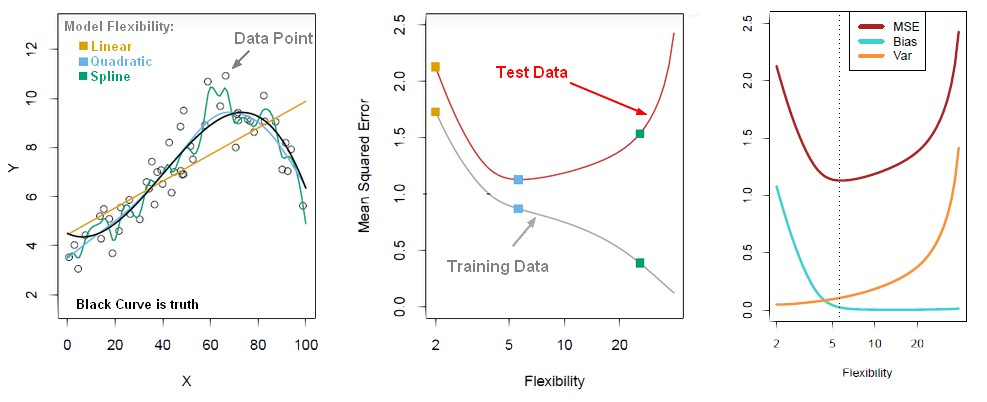
\includegraphics[scale=.3]{bias-variance}
	\begin{itemize}
		\item Simple models give consistent results across test sets (low variance) but don't predict well. (high bias).
		\item Very flexible (complex) models give inconsistent results across test sets (high variance), but do well at prediction (low bias).
	\end{itemize}
\end{frame}

\section*{Classification}

\begin{frame}{Classification}
\begin{align*}
	\text{Error rate: } \frac{1}{n} \sum_{i=1}^{n} \mathbb{I}(y_{i} \neq \hat{y}_{i})
\end{align*}
	\begin{itemize}
		\item Our discussion of MSE previously was in the context of \textit{regression} in which the outcome was a continuous predictor.
		\item There are some slight modifications  that can be made in the setting in which we're interested in prediction \textit{classes:}.
		\item $\{Democrat,Republican\}$, $\{Violent, Nonviolent\}$ , $\{Protest,Non-protest\}$
	\end{itemize}
\end{frame}

\begin{frame}{Classification}
\begin{align*}
	\text{Error rate: } \frac{1}{n} \sum_{i=1}^{n} \mathbb{I}(y_{i} \neq \hat{y}_{i})
\end{align*}
	\begin{itemize}
		\item We are essentially interested in what \% of classifications are correct.
	\end{itemize}
\end{frame}

\begin{frame}{Bayes classifier}

\begin{equation}
 \mathbb{P}(Y = j | X = x_{0})
\end{equation}

	\begin{itemize}
		\item It can be shown that the error rate is minimized by a classifier that assigns each observation a classification based on its predictor value.
	\end{itemize}
\end{frame}

\begin{frame}{Bayes classifier -- text analysis context}

\begin{equation}
 \mathbb{P}(Y = Happy | X = \{depressed, miserable\}) = 0.1
\end{equation}

	\begin{itemize}
		\item Bayes classifiers are used very frequently in text analysis to predict the class of a document given words and other features.
	\end{itemize}
\end{frame}

\begin{frame}{Bayes classifier -- text analysis context -- classification}

\begin{align*}
 \mathbb{P} & (Y = Happy | X = \{depressed, miserable\})  = 0.1 \\
 \mathbb{P} & (Y = Sad | X = \{depressed, miserable\})  = 0.9 \\
  & \argmax_{j} ~\mathbb{P}(Y = j | X = x_{0})
\end{align*}
	\begin{itemize}
		\item Classification proceeds by choosing the class with the highest probability.
		\item In this case \textit{Sad}.
		
	\end{itemize}
\end{frame}

\begin{frame}{Bayes classifier -- text analysis context -- Bayes error}

\begin{align*}
 1-  \E \left( \argmax_{j} ~\mathbb{P}(Y = j | X = x_{0}) \right)
\end{align*}
	\begin{itemize}
		\item If we had two observations in which $ \mathbb{P} (Y = Sad | X) = .9)$ and $ \mathbb{P} (Y = Happy | X) = .6)$.
		\item The Bayes error rate is: $ \frac{0.1 + 0.4}{2} = 0.25$.
		
	\end{itemize}
\end{frame}

\end{document}